\documentclass[oneside, 11pt]{article}

\usepackage[T1]{fontenc}
\usepackage[utf8]{inputenc}
\usepackage[dutch]{babel}

\usepackage{fouriernc}
\usepackage[detect-all, load-configurations=binary,
            separate-uncertainty=true, per-mode=symbol,
            retain-explicit-plus, range-phrase={ tot }]{siunitx}

\usepackage{setspace}
\setstretch{1.2}

\setlength{\parskip}{\smallskipamount}
\setlength{\parindent}{0pt}

\usepackage{geometry}
\geometry{marginparwidth=0.5cm, verbose, a4paper, tmargin=3cm, bmargin=3cm, lmargin=2cm, rmargin=2cm}

\usepackage{float}

\usepackage[fleqn]{amsmath}
\numberwithin{equation}{section}
\numberwithin{figure}{section}

\usepackage{graphicx}
\graphicspath{{Figures/}}
\usepackage{subfig}

\usepackage{tikz}
\usetikzlibrary{plotmarks}

\usepackage{fancyhdr}
\pagestyle{fancy}
\fancyhf{}
\rhead{\thepage}
\renewcommand{\footrulewidth}{0pt}
\renewcommand{\headrulewidth}{0pt}

\usepackage{relsize}
\usepackage{xspace}
\usepackage{url}

\newcommand{\figref}[1]{Figuur~\ref{#1}}

\newcommand{\hisparc}{\textsmaller{HiSPARC}\xspace}
\newcommand{\kascade}{\textsmaller{KASCADE}\xspace}
\newcommand{\sapphire}{\textsmaller{SAPPHiRE}\xspace}
\newcommand{\jsparc}{\textsmaller{jSparc}\xspace}
\newcommand{\hdf}{\textsmaller{HDF5}\xspace}
\newcommand{\aires}{\textsmaller{AIRES}\xspace}
\newcommand{\csv}{\textsmaller{CSV}\xspace}
\newcommand{\python}{\textsmaller{PYTHON}\xspace}
\newcommand{\corsika}{\textsmaller{CORSIKA}\xspace}
\newcommand{\labview}{\textsmaller{LabVIEW}\xspace}
\newcommand{\daq}{\textsmaller{DAQ}\xspace}
\newcommand{\adc}{\textsmaller{ADC}\xspace}
\newcommand{\adcs}{\textsmaller{ADC}s\xspace}
\newcommand{\Adcs}{A\textsmaller{DC}s\xspace}
\newcommand{\hi}{\textsc{h i}\xspace}
\newcommand{\hii}{\textsc{h ii}\xspace}
\newcommand{\mip}{\textsmaller{MIP}\xspace}
\newcommand{\hisparcii}{\textsmaller{HiSPARC II}\xspace}
\newcommand{\hisparciii}{\textsmaller{HiSPARC III}\xspace}
\newcommand{\pmt}{\textsmaller{PMT}\xspace}
\newcommand{\pmts}{\textsmaller{PMT}s\xspace}

\DeclareSIUnit{\electronvolt}{\ensuremath{\mathrm{e\!\!\:V}}}

\DeclareSIUnit{\unitsigma}{\ensuremath{\sigma}}
\DeclareSIUnit{\mip}{\textsmaller{MIP}}
\DeclareSIUnit{\adc}{\textsmaller{ADC}}

\DeclareSIUnit{\gauss}{G}
\DeclareSIUnit{\parsec}{pc}
\DeclareSIUnit{\year}{yr}



\title{Detector plaatsing}
\author{A.P.L.S. de Laat, B. van Eijk}
\docinstallatie{2}{DP}
\version{1.1}

\begin{document}

\maketitle

\textbf{Let op!} Afwijken van de fixatiemethode van de skiboxen is niet
toegestaan!


\section{Planning en veiligheid}

Dit document beschrijft hoe een \hisparc detector op het dak
geïnstalleerd dient te worden. Bij het werken op daken of andere
gevaarlijke locaties moet goed op veiligheid gelet worden. Neem voordat
je begint contact op met de gebouwbeheerder van je school. Die kan
instructies geven over de richtlijnen van het veilig werken op het dak,
en zo is die ook op de hoogte van het werk. Bespreek vooraf wie wat doet
zodat je sneller klaar bent. Check ook of je alle benodigdheden hebt
zodat je niet vaker het dak op en af hoeft.


\section{Detector hanteren}

\textbf{Waarschuwing:} De \hisparc detector met zijn scintillator,
lichtgeleider en \pmt is een fragiel apparaat. Neem daarom de volgende
maatregelen om schade te voorkomen:

\begin{itemize}
    \item Verpak de detector zorgvuldig tijdens transport; de detector
    mag niet kunnen verschuiven in de skibox (voeg extra schuimmateriaal
    toe).
    \item Wanneer de skibox niet horizontaal gehouden kan worden, houd
    de hoge kant van de skibox met de \pmt en kabeldoorvoer, altijd
    boven. Ondersteun de onderkant van de scintillator tegen verschuiven.
    \item Wanneer de detector buiten de skibox verplaatst moet worden,
    zorg er dan voor dat de scintillator en lichtgeleider op voldoende
    plaatsen ondersteund worden om zo breuk in de lijmverbindingen te
    voorkomen.
    \item Voorkom grote schokken aan de \pmt of stoten aan andere
    objecten.
    \item Zorg ervoor dat de kabels netjes uitgerold worden om knikken
    te voorkomen.
    \item Fixeer de \pmt kabels en connectors met tape (bijv. papieren
    schilderstape) op de licht-geleider zodat geen trekbelasting op de
    draden (en \pmt) kan ontstaan.
\end{itemize}

\begin{figure}
    \centering
    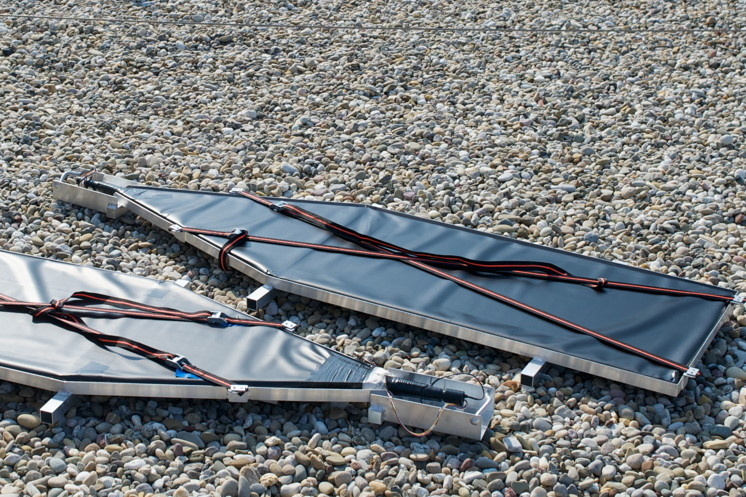
\includegraphics[width=0.47\linewidth]{frames}
    \caption{Detectoren in metalen frames voor vervoer.}
    \label{fig:frames}
\end{figure}


\section{Materiaal lijst}

Hier is een checklist met de benodigde materialen voor een 2 (of 4) detector
station (tussen haken staan de hoeveelheden voor een 4 detector station):

\begin{itemize}
    \item 2 (4) \hisparc detectoren
    \item 2 (4) Coaxkabels van \SI{30}{\meter}
    \item 2 (4) Voedingskabels van \SI{30}{\meter}
    \item 4 (8) Schuimblokken
    \item 2 (4) Skiboxen met kabeldoorvoer
    \item 4 (8) Aluminium kokerprofielen (\SI{200}{\centi\meter} x
    \SI{5}{\centi\meter} x \SI{2.5}{\centi\meter})
    \item 16 (32) Betonnen opsluitbanden (\SI{100}{\centi\meter} x
    \SI{30}{\centi\meter} x \SI{5}{\centi\meter})
    \item Rubberen tegels
    \item \SI{16}{\meter} (\SI{32}{\meter}) 3/4$''$ RVS spanband
    ('Band-it')
    \item 16 (32) 3/4$''$ RVS sluitstukken ('Band-it')
    \item \gps antenne met voet
    \item \gps coaxkabel van \SI{30}{\meter}
    \item Tie-wraps
\end{itemize}

En dit zijn de andere benodigdheden:

\begin{itemize}
    \item Spantang
    \item Hamer
    \item Kniptang
    \item Logboek
    \item Detector draagframes (optioneel)
\end{itemize}


\section{Beschrijving verankering}

De \hisparc detectoren zijn ondergebracht in skiboxen die bij normaal
gebruik geschikt zijn voor toepassing onder uiteenlopende
weersomstandigheden. De boxen verkrijgen hun stabiliteit door ze via hun
standaard bevestigingspunten (4 beugels) vast te zetten en de deksels op
de juiste wijze te sluiten (scharnieren en 3-punts sluiting) en te
vergrendelen (sleutel + slot). Om er voor te zorgen dat de boxen ook
onder extreme weersomstandigheden (storm) op hun plek blijven, is
gekozen voor een robuuste ‘verankering’, te zien in
\figref{fig:schema_verankering}. De verankering bestaat uit 4
opsluitbanden en een aluminium kokerprofiel, dit wordt bij
elkaar gehouden door RVS spanbanden, de skibox is aan het
kokerprofiel verbonden door de standaard bevestigingspunten. Deze
verankering blijft los van het dak zodat er geen aanpassingen aan het
dak zelf noodzakelijk zijn. Het totale gewicht (en dus de lokale
dakbelasting) neemt daardoor wel toe, maar blijft door een goede
gewichtsverdeling beperkt (minder dan
\SI{50}{\kilo\gram\per\square\meter}).

\begin{figure}
    \centering
    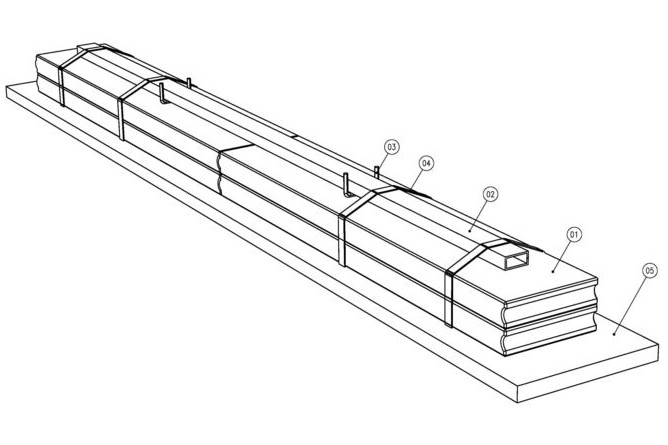
\includegraphics[width=0.7\linewidth]{schema_verankering}
    \caption{Schema van de verankering. 1 - Opsluitbanden, 2 - Aluminium
             kokerprofiel, 3 - Skibox beugels, 4 - Spanband, 5 -
             Rubbertegels.}
    \label{fig:schema_verankering}
\end{figure}

%Voordat de skiboxen met hun detectoren definitief geplaatst kunnen
%worden moeten diverse elektrische tests uitgevoerd worden en moet de
%volledige documentatie voor de opstelling beschikbaar zijn zowel op
%papier als op de lokale (school/instituut) website. Dit is de
%verantwoordelijkheid van de groep leerlingen die aan de bouw en
%plaatsing deelneemt. Met behulp van deze documentatie kunnen de
%resultaten van de individuele metingen aan de scintillator,
%fotoversterkerbuis en uitleeselektronica gecombineerd worden. Dit is
%noodzakelijk om later de signalen van de kosmische straling te kunnen
%interpreteren!


\section{Checklist voor plaatsing}

Voordat de skiboxen geplaatst worden is het raadzaam om de volgende
punten stap voor stap te controleren:

\begin{itemize}
    \item Voorzie iedere detector van een sticker met het stationnummer
    en het detectornummer. Het stationnummer is een uniek
    identificatienummer en wordt ook in software gebruikt en wordt
    aangegeven op de statuspagina van de betreffende cluster op de
    \hisparc website en in het logboek van de detector. Het
    detectornummer wordt bepaald door de poort op het \hisparc kastje
    waar de detector aan verbonden wordt: detectornummers 1 en 2 zijn
    Primary PMT1 en PMT2, detectornummers 3 en 4 zijn Secondary PMT1 en PMT2.
    \item Om te voorkomen dat tijdens het transport de fotobuis
    beschadigt, wordt de detector zo in de skibox geplaatst dat de
    fotoversterkerbuis zich altijd aan de hogere kant van de skibox
    bevindt (aan dezelfde kant als de kabeldoorvoer).
    \item Voor iedere detector is een volledige elektrische test
    uitgevoerd en gedocumenteerd (kopie rapport bij school in het
    logboek, bij coördinerende instelling en geplaatst op lokale
    webpagina’s).
    \item Iedere detector is gekalibreerd (documentatie: in logboek,
    kopie bij school en bij coördinerende instelling en op
    webpagina’s!).
    \item In overleg met gebouwbeheer moet een kabeldoorvoer in het
    gebouw worden aangelegd zodat de kabels van de \hisparc elektronica
    (binnen) naar de detectoren (buiten) kunnen. Onthoudt dat de kabels
    \SI{30}{\meter} lang zijn.
    \item 1 signaalkabel (coax) en 1 voedingkabel (5-aders) per skibox
    zijn getest en aangelegd. Zorg dat de kabels aan beide uiteinden
    voorzien zijn van het betreffende detectornummer. Let op bij de
    aanleg: de voedingskabels zijn niet symmetrisch, de uiteinden hebben
    verschillende connectors (male/female)! De fotobuis bezit een ‘male’
    connector en moet dus verbonden worden met de ‘female’ connector van
    de voedingskabel en de 'male' connector van de kabel moet verbonden
    worden met de 'female' connector van de \hisparc elektronica.
    \item De kabels in de ‘vrije natuur’ (op het dak en langs de gevel)
    zijn bij voorkeur in vast gemonteerde (metalen/kunststoffen)
    kabelgoten/buizen ondergebracht (de voedingsspanning van de fotobuis
    bedraagt \SI{12}{\volt} met beperkte belastbaarheid). Voorkom
    kortsluiting; bescherm de connectors tegen mechanische belasting en
    inwerking van vocht en voorkom scherpe knikken in de kabels!
    \item Er wordt rekening gehouden met speciale
    voorschriften/voorzieningen bij dakbeveiliging tegen blikseminslag.
\end{itemize}


\section{Positie van detectoren en \gps antenne}

Twee verschillende \hisparc detector configuraties worden toegepast; een
twee-skibox opstelling en een vier-skibox opstelling.


\subsection{Twee detectoren}

De opstelling met twee skiboxen is bij uitstek geschikt wanneer het
station gecombineerd wordt met andere stations in de directe omgeving
(cluster centra). Het totale detectieoppervlak van dit station bedraagt
$0.5 + 0.5 = \SI{1}{\square\meter}$. Om de hoekafhankelijkheid van de
opstelling te beperken, worden beide skiboxen parallel geplaatst (de
effectieve ‘lengte’ van het station in twee richtingen is dan
\SI{1}{\meter}). De ‘typische’ afstand tussen de twee skiboxen bedraagt
5 à 6 meter. Zie \figref{fig:station-2-layout} voor een schematische
weergave van deze opstelling.

De \gps kan tussen de twee skiboxen op de hartlijn van de scintillatoren
geplaatst worden. Meet de Noord-Zuid oriëntatie van deze hartlijn met
een kompas en maak een situatieschets waarin deze hoek (t.o.v. noorden)
en de afstanden tussen de \gps en detectoren duidelijk is.

\begin{figure}
    \centering
    % Based on station-layout.tex from Fokkema 2013.

\begin{tikzpicture}
    [ font=\sffamily, x=.75cm, y=.75cm,
      hisparc/.style={draw},
    ]
    \foreach \sx / \sy / \angle in {-3/0/180, 3/0/180} {
        \begin{scope}[hisparc, shift={(\sx,\sy)}, rotate=\angle]
            \draw[rounded corners=2.25pt]
                (-.4, .7) .. controls (0, .75) ..  (.4, .7) -- 
                (.35, -1.7) ..  controls(0, -1.72) ..  (-.35, -1.7) --
                cycle;
            \draw (-.25, .5) rectangle (.25, -.5);
            \draw (-.25, -.5) -- (-.02, -1) --(.02, -1) -- (.25, -.5);
            \fill (-.02, -1) rectangle (.02, -1.2);
        \end{scope}
    }
    \draw[fill] (0, 0) circle (.10) node [above] {GPS};
    \node[color=gray] at (-3.75, .75) {\Large 1};
    \node[color=gray] at (2.25, .75) {\Large 2};

    \coordinate (A) at (-3, 0);
    \coordinate (B) at (3, 0);
    \coordinate (A') at ($ (A)!.8cm!-90:(B) $);
    \coordinate (B') at ($ (B)!.8cm!90:(A) $);
    \draw (A) -- ($ (A)!1.1!(A') $);
    \draw (B) -- ($ (B)!1.1!(B') $);
    \draw[<->] (A') -- (B') node [midway, below] {\SI{6}{\meter}};

    \coordinate (E) at (0, 0);

    \draw[dashed,gray] (A) -- (B);
\end{tikzpicture}

    \caption{Schematische weergave van de plaatsing van de detectoren in een
             2-detector station met een \gps in het midden. De afstand
             tussen de scintillatoren is ongeveer \SI{6}{\meter}.}
    \label{fig:station-2-layout}
\end{figure}


\subsection{Vier detectoren}

Een opstelling met 4 detectoren biedt de mogelijkheid om de richting van
een lokale deeltjeslawine te bepalen. Ook hier is gekozen voor een
opstelling waarbij de geometrie geoptimaliseerd is voor symmetrie; de
vier detectoren vormen de hoekpunten van een ruit (met zijden van
\SI{10}{\meter}), zie \figref{fig:station-4-layout}. Wanneer in alle
vier de detectoren een signaal gemeten wordt, kunnen in totaal 4
driehoeken onderscheiden worden; richting reconstructie van de kosmische
straling kan zo 4 keer uitgevoerd en op consistentie getest worden.

De \gps kan in het midden op de hartlijn tussen de scintillatoren 3 en 4
geplaatst worden. Ook hier moet een detailschets gemaakt worden van de
positie (afstanden en richting) van de detectoren ten opzichte van de
\gps. Hier moet de oriëntatie van de hartlijn tussen 3 en 4 t.o.v.
het Noorden met een kompas bepaald worden. De volgorde in de nummering
van de detectoren is eenduidig en mag niet veranderd worden (Primary:
scintillator 1 en 2 en Secondary: scintillator 3 en 4). Noteer in de schets
duidelijk welke detector welk nummer heeft!

\begin{figure}
    \centering
    % Based on station-layout.tex from Fokkema 2013.

\begin{tikzpicture}
    [ font=\sffamily, x=.75cm, y=.75cm,
      hisparc/.style={draw},
    ]
    \foreach \sx / \sy / \angle in {-5/0/90, 5/0/-90, 10/8.66/0, 0/8.66/0} {
        \begin{scope}[hisparc, shift={(\sx,\sy)}, rotate=\angle]
            \draw[rounded corners=2.25pt]
                (-.4, .7) .. controls (0, .75) ..  (.4, .7) -- 
                (.35, -1.7) ..  controls(0, -1.72) ..  (-.35, -1.7) --
                cycle;
            \draw (-.25, .5) rectangle (.25, -.5);
            \draw (-.25, -.5) -- (-.02, -1) --(.02, -1) -- (.25, -.5);
            \fill (-.02, -1) rectangle (.02, -1.2);
        \end{scope}
    }
    \draw[fill] (0, 0) circle (.10) node [above] {GPS};
    \node[color=gray] at (-.75, 8.1) {\Large 1};
    \node[color=gray] at (9.25, 8.1) {\Large 2};
    \node[color=gray] at (-5, .75) {\Large 3};
    \node[color=gray] at (5, .75) {\Large 4};

    \coordinate (A) at (-5, 0);
    \coordinate (B) at (5, 0);
    \coordinate (A') at ($ (A)!.8cm!-90:(B) $);
    \coordinate (B') at ($ (B)!.8cm!90:(A) $);
%    \draw (A) -- ($ (A)!1.1!(A') $);
%    \draw (B) -- ($ (B)!1.1!(B') $);
%    \draw[<->] (A') -- (B') node [midway, below] {\SI{10}{\meter}};

    \coordinate (D) at (0, 8.66);
    \coordinate (C') at ($ (A)!.8cm!90:(D) $);
    \coordinate (D') at ($ (D)!.8cm!-90:(A) $);
    \draw (A) -- ($ (A)!1.1!(C') $);
    \draw (D) -- ($ (D)!1.1!(D') $);
    \draw[<->] (C') -- (D') node [midway, above, sloped] {\SI{10}{\meter}};

    \coordinate (E) at (0, 0);
    \coordinate (F) at (10, 8.66);
    \coordinate (D'') at ($ (D)!.8cm!180:(E) $);
    \coordinate (E') at ($ (E)!.8cm!90:(A) $);
    \coordinate (F') at ($ (F)!.8cm!-90:(D) $);
%    \draw (F) -- ($ (F)!1.1!(F') $);
%    \draw (D) -- ($ (D)!1.1!(D'') $);
%    \draw[<->] (F') -- (D'') node [midway, below, sloped] {\SI{10}{\meter}};
    \draw (A) -- ($ (A)!1.1!(A') $);
    \draw (E) -- ($ (E)!1.1!(E') $);
    \draw[<->] (A') -- (E') node [midway, below] {\SI{5}{\meter}};

    \draw[<->] (A) ++(0:2.1) arc (0:60:2.1);
    \node at (-2.8, 1.4) {60°};

    \draw[dashed,gray] (A) -- (B);
    \draw[dashed,gray] (A) -- (D);
    \draw[dashed,gray] (B) -- (D);
    \draw[dashed,gray] (B) -- (F);
    \draw[dashed,gray] (F) -- (D);
%    \draw[dashed,gray] (A) -- (F);
\end{tikzpicture}

    \caption{Schematische weergave van de plaatsing van de detecoren in een
             4-detector station. De detectoren liggen in de vorm van een
             ruit, dus twee aaneengesloten gelijkzijdige driehoeken met
             zijden van \SI{10}{\meter}. De \gps is geplaatst tussen
             detector 3 en 4.}
    \label{fig:station-4-layout}
\end{figure}


\section{Plaatsing van de skiboxen}

\textbf{Let op!} Denk aan de voorschriften m.b.t. werken op daken (o.a.
blijf meer dan 2 meter van de dakrand verwijderd!). Informeer bij de
gebouwbeheerder voor alle regels.

\begin{itemize}
    \item Wees extreem voorzichtig met de detector; de lijmverbindingen
    (scintillator/lichtgeleider, lichtgeleider/fotobuis) zijn fragiel
    en kunnen snel breken waardoor de kostbare fotobuis onherstelbaar
    beschadigd kan raken.
    \item Zorg dat in ieder skibox één gat geboord is voor de
    kabeldoorvoer. De kabeldoorvoer moet van binnen worden aangebracht,
    zodat alleen de bevestigingsmoer zich aan de buitenzijde bevindt.
    \item Geen extra gewichten in de skibox plaatsen.
    \item Verwijder het schuimmateriaal dat voor transport
    boven de scintillatieplaat en lichtgeleider aan is gebracht pas
    dan wanneer de skibox op zijn definitieve plek geplaatst is.
    \item Let op dat bij het transport van de skiboxen deze op de juiste
    wijze (3 punten!) gesloten zijn (en op slot!) terwijl voldoende
    schuimmateriaal is aangebracht om het verschuiven van de
    scintillatieplaat en lichtgeleider te voorkomen (laat de sleutel
    nooit in het slot van de skibox zitten, de sleutel kan eenvoudig
    afbreken!).
\end{itemize}

De skiboxen worden gefixeerd via hun standaard bevestigingspunten zodat
de belasting van de bevestigingspunten identiek is aan de belasting op
een autodak. Alleen zo kan veilige montage gegarandeerd worden. Kies de
uiterste positie (zo ver mogelijk van elkaar af) van de
bevestigingspunten in de skibox. Er worden een aantal series skiboxen
toegepast die qua afmetingen niet veel verschillen, maar wel afwijken in
de manier waarop de bevestigingsbeugels in de box gefixeerd worden.


\subsection{Hapro skiboxen}

Bij elke Hapro skibox worden 4 beugels en 4 beugelvergrendelingen
geleverd. In \figref{fig:beugels_hapro} is de vergrendeling in
‘ontgrendelde’ toestand weergegeven, zo kunnen de uiteinden van de
beugels door de onderkant van de skibox erdoor worden gestoken. Door dan
het centrale deel rechtsom te draaien worden de beugels vastgeklemd en
kan de rode zekering over het uiteinde van het draaiende deel geschoven
worden.

\begin{figure}
    \centering
    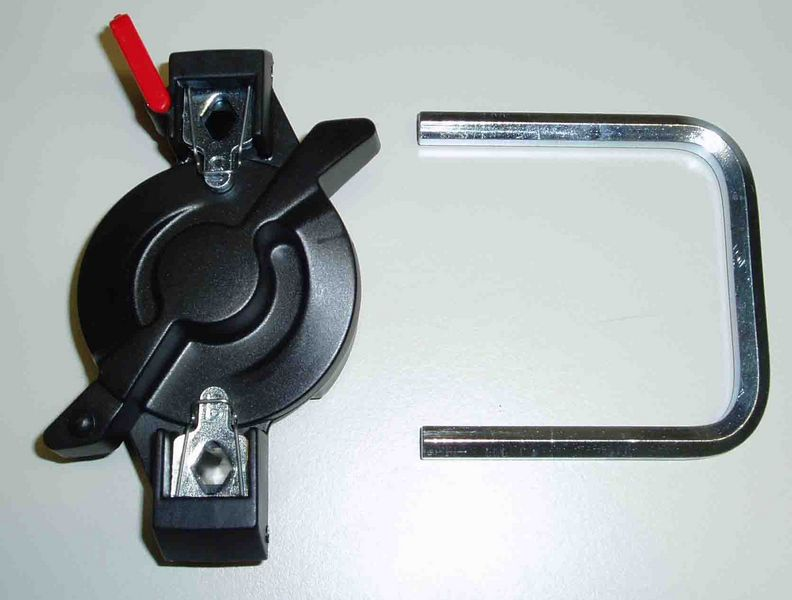
\includegraphics[width=0.47\linewidth]{beugels_hapro}
    \caption{Bevestigingbeugels en vergrendeling van de Hapro skiboxen.}
    \label{fig:beugels_hapro}
\end{figure}


\subsection{Thule skiboxen}

Bij de Thule skibox worden 4 beugels, 8 moeren, en een aantal
afdekplaatjes geleverd (\figref{fig:beugels_thule}). De beugels worden van onder in de gaten in de
bodem van de skibox geplaatst. Vervolgens worden aan de binnenzijde van
de box de rubberen en kunststof afdekplaat (in deze volgorde!) over de
uiteinden van de beugel geschoven. Tenslotte worden de moeren op de
uiteinden van de beugel gedraaid. De niet gebruikte gaten in de bodem
van de skibox worden met meegeleverde (zwarte) plastic stickers afgedekt.

\begin{figure}
    \centering
    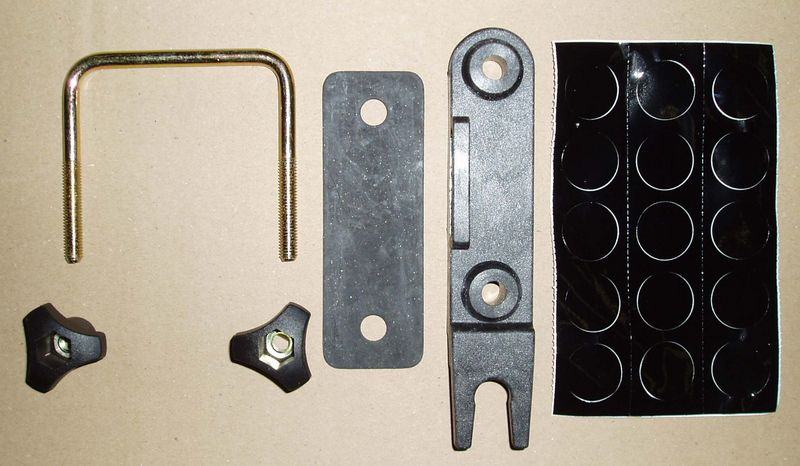
\includegraphics[width=0.47\linewidth]{beugels_thule}
    \caption{Bevestigingbeugels, moeren en afdekplaatjes van de Thule
             skiboxen.}
    \label{fig:beugels_thule}
\end{figure}


\subsection{Verankering skiboxen}

Dit beschrijft de ‘verankering’ van één skibox op het dak. Afwijken van
deze methode is niet zonder overleg toegestaan!

Afhankelijk van de dakbedekking kunnen rubberen matten of een aantal
rubberen tegels aangebracht worden waarop de betonnen opsluitbanden
geplaatst worden. Het RVS band wordt met een spantang om de kokerbalk en
betonnen opsluitbanden gesnoerd. De kokerbalken drukken de twee beugels
tegen de opsluitbanden. De beugels steken door de bodem van de skibox.
De vergrendelingen/moeren op de beugels aan de binnenzijde van de skibox
zorgen ervoor dat de skibox op de kokerbalk gefixeerd wordt. Het
sluitstuk van de spanband is eveneens van RVS en heeft vertandingen en
sluitnokken waarmee de band gefixeerd wordt (\figref{fig:spanband}). Met
de spantang wordt de spanband strak om de opsluitbanden en het
kokerprofiel getrokken, zo dat het sluitstuk op het kokerprofiel blijft
(\figref{fig:spanband_spannen}). Buig de spanband zodat het losse stuk
met de nokken vast gezet kan worden (\figref{fig:spanband_buigen}). De
nokken worden met een hamer om de band ‘gebogen’
(\figref{fig:spanband_verankeren}). De spantang heeft een ingebouwde
schaar waarmee de band op lengte kan worden geknipt. Per skibox worden
zo 8 spanbanden aangebracht.

\begin{figure}
    \centering
    \subfloat[]{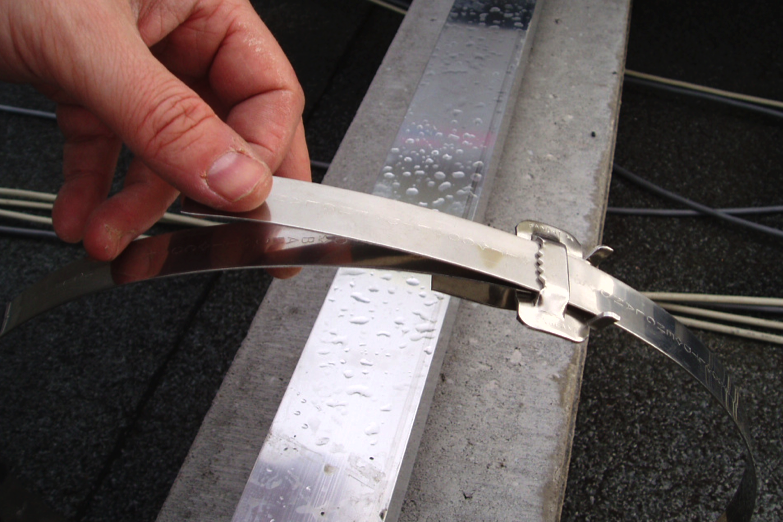
\includegraphics[width=0.47\linewidth]{spanband}
                \label{fig:spanband}}
    \subfloat[]{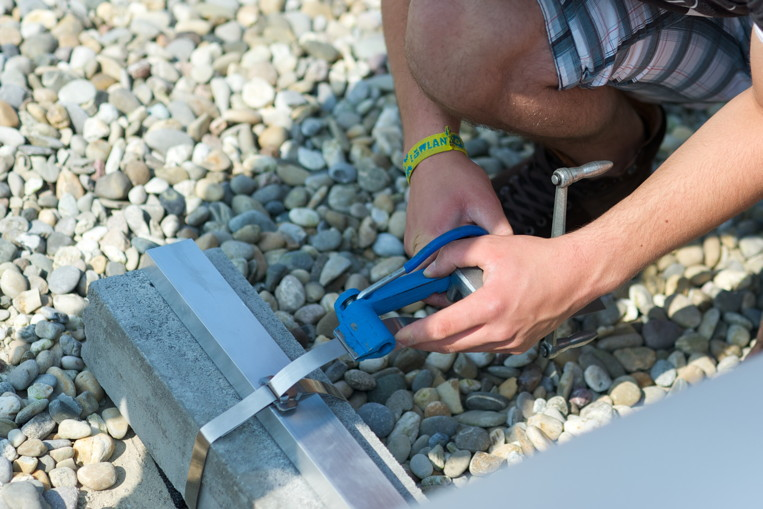
\includegraphics[width=0.47\linewidth]{spanband_spannen}
                \label{fig:spanband_spannen}}
    \caption{Doorvoeren van spanband sluitstukken. Spannen van de
             spanbanden.}
\end{figure}

\begin{figure}
    \centering
    \subfloat[]{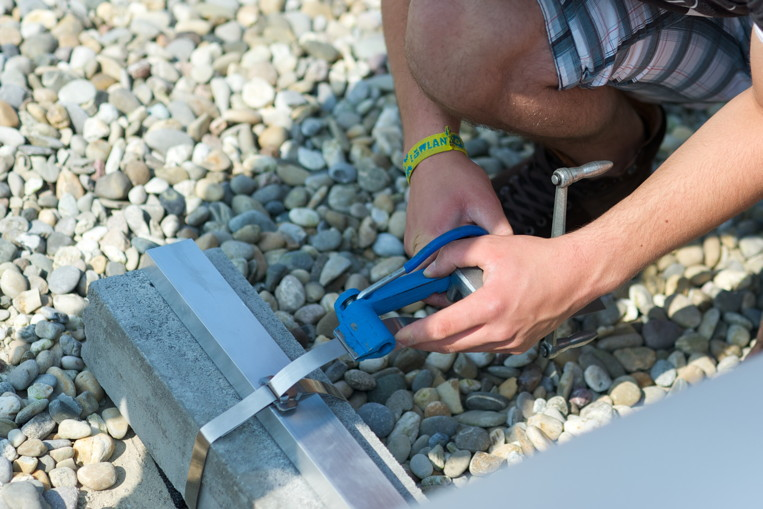
\includegraphics[width=0.47\linewidth]{spanband_buigen}
                \label{fig:spanband_buigen}}
    \subfloat[]{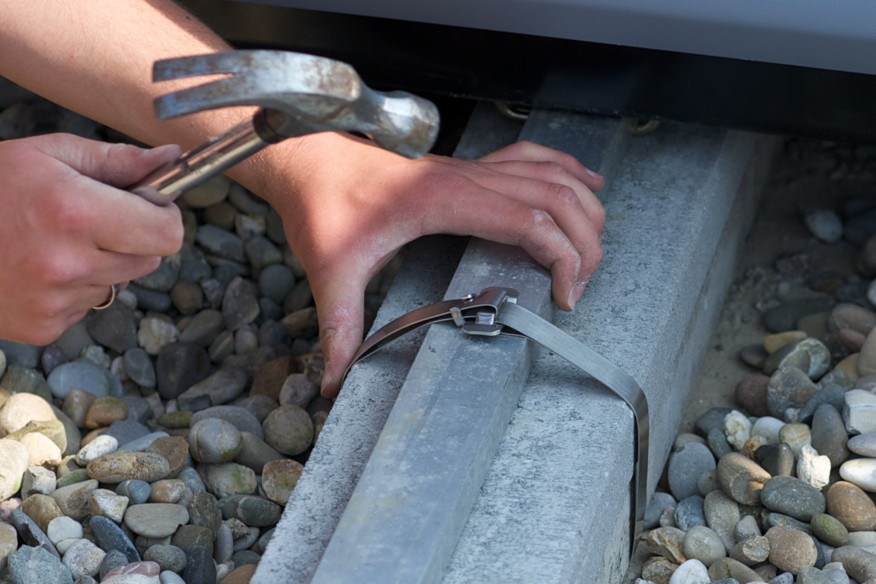
\includegraphics[width=0.47\linewidth]{spanband_verankeren}
                \label{fig:spanband_verankeren}}
    \caption{Ombuigen spanband. Verankeren van de spanband.}
\end{figure}

Let op dat de kabelgoten zo dicht mogelijk bij de skibox eindigen en dat
de kabels langer zijn dan strikt noodzakelijk om de connectors van de
fotobuizen te bereiken. Deze extra kabellengte wordt los in de skibox
(rond de scintillatorplaat) ondergebracht zodat een eenvoudige
‘trekontlasting’ van de kabel aan de fotobuis ontstaat (zie
\figref{fig:detector_in_skibox}). De kabels worden bij de kabeldoorvoer
in de skibox voorzien van twee extra tiewarps (die niet afgeknipt
worden!). Zo wordt een extra trekontlasting verkregen. De kabels kunnen
door een PVC buis (zie \figref{fig:kabel_doorvoer}) of andere kabel
doorvoer het gebouw binnen komen, overleg hierover met gebouwbeheer.
Iedere detectieopstelling bezit twee sets sleutels. Een set wordt
beheerd door de school (blauw label); de reservesleutels worden beheerd
door de clustercoördinator (rood label).

\begin{figure}
    \centering
    \subfloat[]{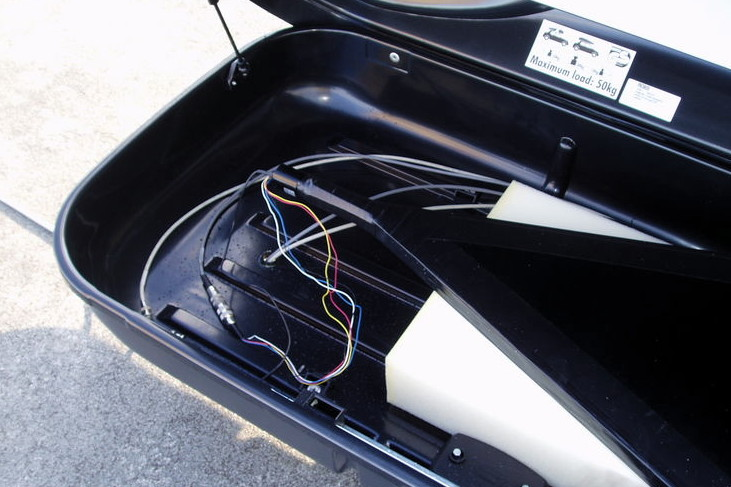
\includegraphics[width=0.47\linewidth]{detector_in_skibox}
                \label{fig:detector_in_skibox}}
    \subfloat[]{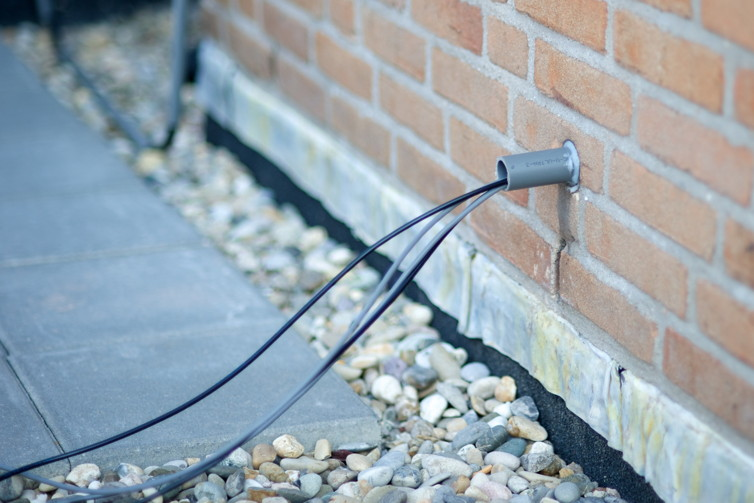
\includegraphics[width=0.47\linewidth]{kabel_doorvoer}
                \label{fig:kabel_doorvoer}}
    \caption{Doorvoer in de muur voor de kabels. Kabels komen de skibox
             binnen.}
\end{figure}

Tenslotte, het is uiterst belangrijk dat het deksel van de skibox op de
juiste wijze - d.w.z. het deksel sluit aan alle randen terwijl de
sleutel zonder veel kracht uit te oefenen omgedraaid kan worden -
gesloten wordt! Uiteraard moet er geen schuim bovenop de
scintillator en de lichtgeleider in de skibox achterblijven.

\textbf{Disclaimer} - de hier beschreven plaatsingsmethode is ontwikkeld
op basis van de gegevens verstrekt door de fabrikant van de skiboxen en
is geverifieerd door constructeurs. De methode heeft zich in de praktijk
bewezen. Op enigerlei wijze afwijken van deze methode geschiedt
uitdrukkelijk op eigen verantwoordelijkheid en wordt ten sterkste
ontraden!


\section{\gps plaatsing}

De \gps antenne wordt op een stabiele mast of antennevoet in de directe
nabijheid van de detectoren geplaatst, zodat de antenne ‘vrij
zicht’ heeft op een zo groot mogelijk deel van de hemel. Bij correcte
plaatsing, worden meer dan 5 satellieten gelijktijdig waargenomen.

De \gps antennekabel heeft aan beide zijden dezelfde connector.

Bij voorkeur wordt de \gps antenne gemonteerd op een stoeptegel met
behulp van de bijgeleverde kunststof voet. Doe de voet over de \gps
antennekabel en bevestig de kabel aan de \gps antenne, schroef dan de
voet op de \gps antenne. Boor in de stoeptegel 3 gaten die passen met de
plek van de gaten in de \gps voet. Gebruik dan lange RVS bouten met
moeren om de voet aan de stoeptegel vast te maken zodat er genoeg ruimte
onder de voet is zodat de antennekabel niet knikt. Zie
\figref{fig:gps_stoeptegel} voor een voorbeeld hiervan. De \gps antenne
kan ook op een buis gemonteerd worden, de onderzijde past op een
gasfitting van 3⁄4$''$.

\begin{figure}
    \centering
    \subfloat[]{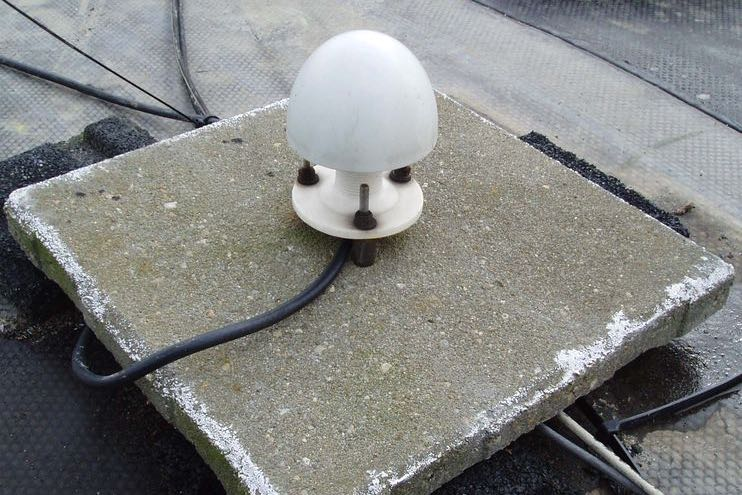
\includegraphics[width=0.47\linewidth]{gps_stoeptegel}
                \label{fig:gps_stoeptegel}}
    \subfloat[]{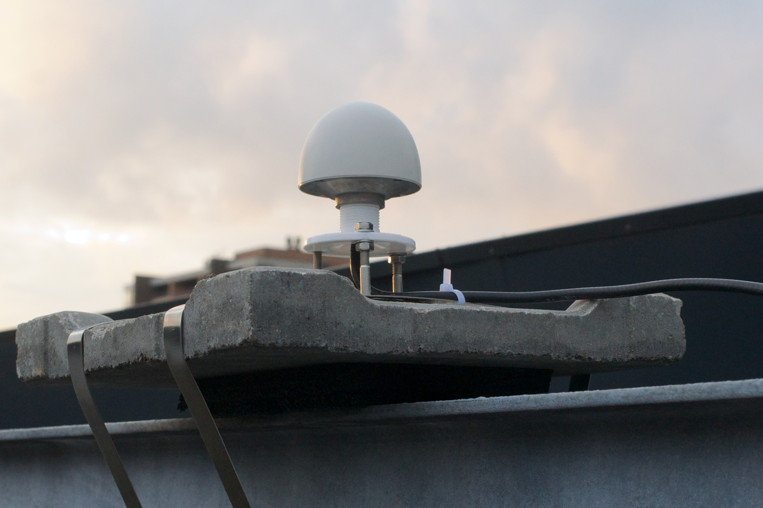
\includegraphics[width=0.47\linewidth]{gps_stoeptegel_alt}
                \label{fig:gps_stoeptegel_alt}}
    \caption{\gps bevestigd op voet. Een hoger geplaatste \gps geeft
             soms beter zicht van de hemel.}
\end{figure}

De \gps antennekabel wordt bij voorkeur in een stabiele kabelgoot
gemonteerd (de \gps kabellengte bedraagt eveneens \SI{30}{\meter}; deze
kabellengte mag zonder speciale maatregelen niet veranderd worden!). De
kabel mag niet los liggen/hangen, vooral niet langs een mast (gebruik
tiewraps)!


\section{Afronding}

Zorg dat er geen rommel achter blijft op het dak, zoals lossen stukken
spanband. Vergeet ook niet de skiboxen goed op slot te doen en de
sleutels op een goede plek te bewaren.

\begin{figure}
    \centering
    \subfloat[]{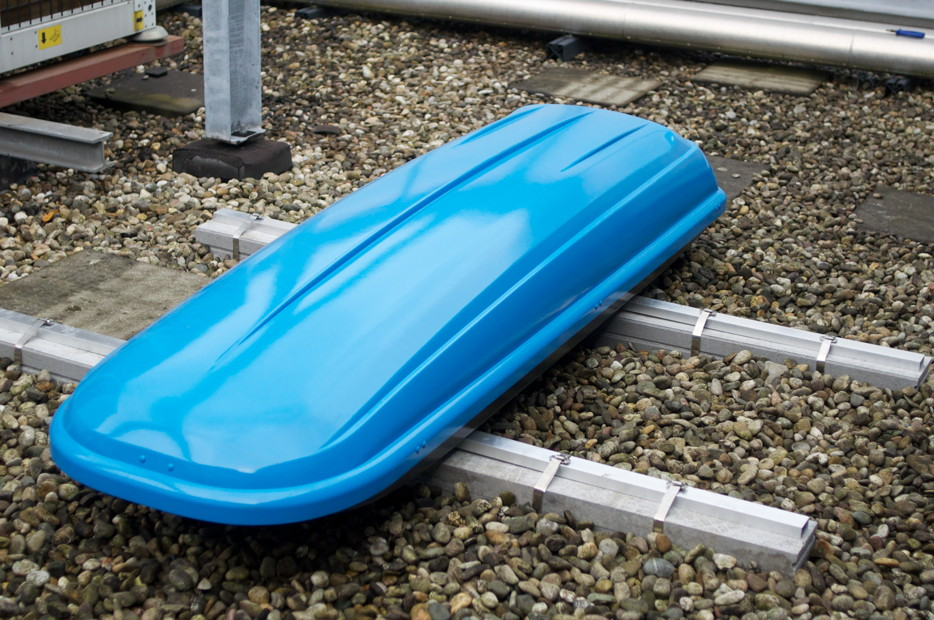
\includegraphics[width=0.47\linewidth]{klaar_skibox}
                \label{fig:klaar_skibox}}
    \subfloat[]{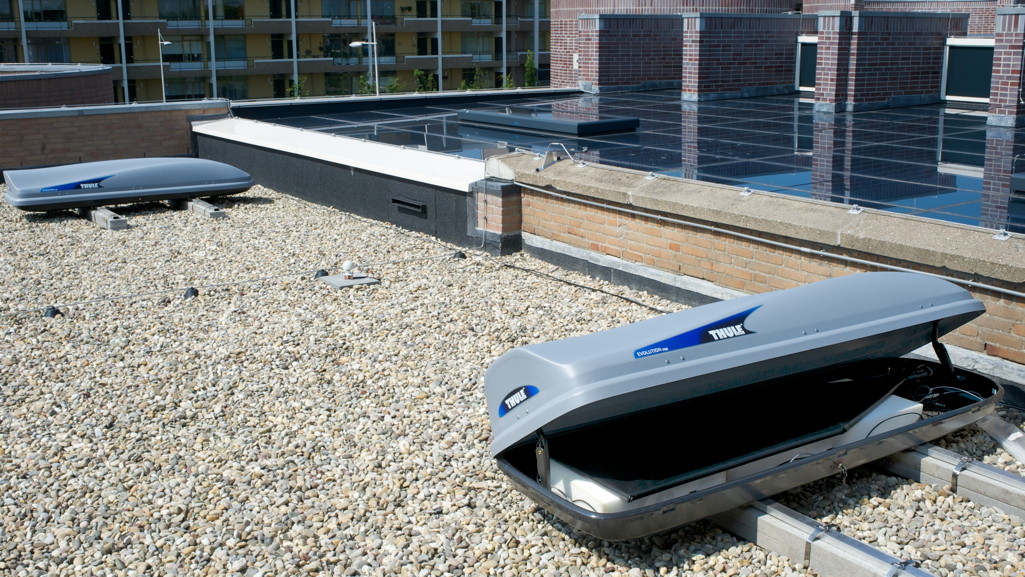
\includegraphics[width=0.47\linewidth]{klaar_station}
                \label{fig:klaar_station}}
    \caption{Geïnstaleerde detector stations. Vergeet niet de skiboxen
             op slot te doen.}
\end{figure}

Nu de detectoren geplaatst zijn kan het meten beginnen, hiervoor moet de
\hisparc elektronica aan de pc en detectoren verbonden worden. De
documentatie die de software installatie beschrijft is online te vinden
op \url{http://docs.hisparc.nl/station-software/doc/index.html}.


%\begin{thebibliography}{9}
%\end{thebibliography}

\end{document}
